%
% mountain.tex
%
\section{Chart::Mountain}
\name{Chart::Mountain}
\file{Mountain.pm}
\requires{Chart::Base, GD, Carp, FileHandle}
\begin{Description} 
\class{Mountain} is a subclass of Chart::Base.
The class Mountain creates a mountain chart.
\end{Description}

\parindent 0pt{\large Example:}
\begin{figure}[h]
	\begin{center}
		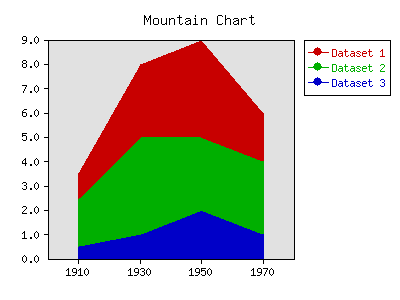
\includegraphics[scale =0.6]{mountain.png}
	\end{center}
	\caption{Mountain chart}
	\label{fig:mountain}
\end{figure}
\begin{verbatim}
use Chart::Mountain;

$g = Chart::Mountain->new();

@data = [ [1910, 1930, 1950, 1970],
          [1, 3, 4, 2],
          [2, 4, 3, 3],
          [0.5, 1, 2, 1]];

$g->set('title' => 'Mountain Chart',
        'grid_lines' => 'false',
        'precision' => 1);

$g->png("mountain.png", @data);
\end{verbatim}

\begin{Constructor} 
An instance of a mountain chart object can be created with the constructor \textit{new()}:
\begin{quote}
\fett{\$obj = Chart::Mountain->new();}\\
\fett{\$obj = Chart::Mountain->new(\kursiv{width}, \kursiv{height});}
\end{quote}
If \textit{new()} has no arguments, 
the constructor returns an image with the size 300x400 pixels. If \textit{new()} 
has two arguments \parameter{width} and \parameter{height}, 
it returns an image with the desired size.
\end{Constructor}


\Methods
\method{All universal valid methods, see page \pageref{methods}
of \class{Chart::Base}.} \\[\parabstand]
%
\Attributes
All universal valid options, see page \pageref{options}. 
Also available, these special options:
\begin{description}
\item['y\_axes'] Tells chart where to place the y-axis. 
                Valid values are 'left', 'right' and 'both'. Defaults to 'left'.
\end{description}
